\chapter{Controlling the code generation}
Several options of the \faust compiler allow to control the generated C++ code. By default the computations are done sample by sample in a single loop. But the compiler can also generate \textit{vector} and \textit{parallel} code.

\section{Vector code generation}
Modern C++ compilers are able to do autovectorization, that is to use SIMD instructions to speedup the code. These instructions can typically operate in parallel on short vectors of 4 simple precision floating point numbers thus leading to a theoretical speedup of $\times4$. 
Autovectorization of C/C++ programs is a difficult task. Current compilers are very sensitive to the way the code is arranged. In particular too complex loops can prevent autovectorization. The goal of the vector code generation is to rearrange the C++ code in a way that facilitates the autovectorization job of the C++ compiler. Instead of generating a single sample computation loop, it splits the computation into several simpler loops that communicates by vectors.

The vector code generation is activated by passing the \lstinline!--vectorize! (or \lstinline!-vec!) option to the \faust compiler. Two additional options are available:  \lstinline!--vec-size <n>! controls the size of the vector (by default 32 samples) and \lstinline!--loop-variant 0/1! gives some additional control on the loops.  

To illustrate the difference between scalar code and vector code, let's take the computation of the RMS (Root Mean Square) value of a signal.  Here is the \faust code that computes the Root Mean Square of a sliding window of 1000 samples:
\label{rms}
\begin{lstlisting}
// Root Mean Square of n consecutive samples
RMS(n) = square : mean(n) : sqrt ;

// Square of a signal
square(x) = x * x ;

// Mean of n consecutive samples of a signal
// (uses fixpoint to avoid the accumulation of
// rounding errors) 
mean(n) = float2fix : integrate(n) : 
          fix2float : /(n); 

// Sliding sum of n consecutive samples
integrate(n,x) = x - x@n : +~_ ;

// Convertion between float and fix point
float2fix(x) = int(x*(1<<20));      
fix2float(x) = float(x)/(1<<20);    

// Root Mean Square of 1000 consecutive samples
process = RMS(1000) ;
\end{lstlisting}

The compute() method generated in scalar mode is the following:

\begin{lstlisting}
virtual void compute (int count, 
                      float** input, 
                      float** output) 
{
  float* input0 = input[0];
  float* output0 = output[0];
  for (int i=0; i<count; i++) {
    float fTemp0 = input0[i];
    int iTemp1 = int(1048576*fTemp0*fTemp0);
    iVec0[IOTA&1023] = iTemp1;
    iRec0[0] = ((iVec0[IOTA&1023] + iRec0[1])
                    - iVec0[(IOTA-1000)&1023]);
    output0[i] = sqrtf(9.536744e-10f * 
                       float(iRec0[0]));
    // post processing
    iRec0[1] = iRec0[0];
    IOTA = IOTA+1;
  }
}
\end{lstlisting}

The \lstinline!-vec! option leads to the following reorganization of the code:
\begin{lstlisting}
virtual void compute (int fullcount, 
                      float** input, 
                      float** output) 
{
  int     iRec0_tmp[32+4];
  int*    iRec0 = &iRec0_tmp[4];
  for (int index=0; index<fullcount; index+=32) 
  {
    int count = min (32, fullcount-index);
    float* input0 = &input[0][index];
    float* output0 = &output[0][index];
    for (int i=0; i<4; i++) 
      iRec0_tmp[i]=iRec0_perm[i];
    // SECTION : 1
    for (int i=0; i<count; i++) {
      iYec0[(iYec0_idx+i)&2047] =
               int(1048576*input0[i]*input0[i]);
    }
    // SECTION : 2
    for (int i=0; i<count; i++) {
      iRec0[i] = ((iYec0[i] + iRec0[i-1]) - 
               iYec0[(iYec0_idx+i-1000)&2047]);
    }
    // SECTION : 3
    for (int i=0; i<count; i++) {
      output0[i] = sqrtf((9.536744e-10f * 
                 float(iRec0[i])));
    }
    // SECTION : 4
    iYec0_idx = (iYec0_idx+count)&2047;
    for (int i=0; i<4; i++)
      iRec0_perm[i]=iRec0_tmp[count+i];
  }
}
\end{lstlisting}

While the second version of the code is more complex, it turns out to be much easier to vectorize efficiently by the C++ compiler. Using Intel icc 11.0, with the exact same compilation options: \texttt{-O3 -xHost -ftz -fno-alias -fp-model fast=2}, the scalar version leads to a throughput performance of 129.144  MB/s, while the vector version achieves 359.548  MB/s, a speedup of x2.8 ! 

\begin{figure}[htb]
  \centering
  \includegraphics[scale=0.75]{images/compiler-stack}
  \caption{\faust's stack of code generators}   
  \label{fig:stack}
\end{figure}

The vector code generation is built on top of the scalar code generation (see figure \ref{fig:stack}). Every time an expression needs to be compiled, the compiler checks if it requires a separate loop or not. It applies some simple rules for that. Expressions that are shared (and are complex enough) are good candidates to be compiled in a separate loop, as well as recursive expressions and expressions used in delay lines. 

The result is a directed graph in which each node is a computation loop (see Figure \ref{fig:loopgraph}). This graph is stored in the klass object and a topological sort is applied to it before printing the code. 

\begin{figure}[htb]
  \centering
  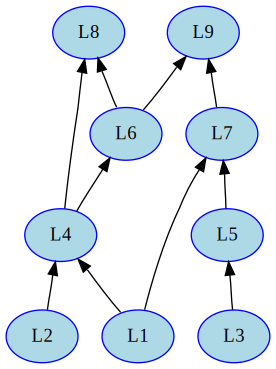
\includegraphics[scale=0.75]{graphs/loopgraph2}
  \caption{The result of the -vec option is a directed acyclic graph (DAG) of small computation loops}   
  \label{fig:loopgraph}
\end{figure}

\section{Parallel code generation}

The parallel code generation is activated by passing either the \lstinline!--openMP! (or \lstinline!-omp!) option or the \lstinline!--scheduler! (or \lstinline!-sch!) option. It implies the \lstinline!-vec! options as the parallel code generation is built on top of the vector code generation.  

\subsection{The OpenMP code generator}

\begin{figure}[htb]
  \centering
  \includegraphics[scale=0.5,angle=-90]{images/openmp-model}
  \caption{OpenMP is based on a fork-join model}   
  \label{fig:openmp}
\end{figure}

The \lstinline!--openMP! (or \lstinline!-omp!) option given to the \faust compiler will insert appropriate OpenMP directives in the C++ code. OpenMP (http://wwww.openmp.org) is a well established API that is used to explicitly define direct multi-threaded, shared memory parallelism. It is based on a fork-join model of parallelism (see figure \ref{fig:openmp}). 
Parallel regions are delimited by \lstinline!#pragma omp parallel! constructs. At the entrance of a parallel region a team of parallel threads is activated. The code within a parallel region is executed by each thread of the parallel team until the end of the region. 

\begin{lstlisting}
#pragma omp parallel
{
  // the code here is executed simultaneously by 
  // every thread of the parallel team
  ...
}
\end{lstlisting}

In order not to have every thread doing redundantly the exact same work, OpemMP provides specific \textit{work-sharing} directives. For example \lstinline!#pragma omp sections! allows to break the work into separate, discrete sections, each section being executed by one thread:

\begin{lstlisting}
#pragma omp parallel
{
  #pragma omp sections
  {
    #pragma omp section
    {
      // job 1
    }
    #pragma omp section
    {
      // job 2
    }
    ...
  }

  ...
}
\end{lstlisting}

\subsection{Adding OpenMP directives}
As said before the parallel code generation is built on top of the vector code generation. The graph of loops produced by the vector code generator is topologically sorted in order to detect the loops that can be computed in parallel. The first set $S_0$ (loops $L1$, $L2$ and $L3$ in the DAG of Figure \ref{fig:loopgraph}) contains the loops that don't depend on any other loops, the set $S_1$ contains the loops that only depend on loops of $S_0$, (that is loops $L4$ and $L5$), etc.. 

As all the loops of a given set $S_n$ can be computed in parallel, the compiler will generate a \lstinline!sections! construct with a \lstinline!section! for each loop. 
\begin{lstlisting}
  #pragma omp sections
  {
    #pragma omp section
    for (...) {
      // Loop 1
    }
    #pragma omp section
    for (...) {
      // Loop 2
    }
    ...
  }
\end{lstlisting}
 
If a given set contains only one loop, then the compiler checks to see if the loop can be parallelized (no recursive dependencies) or not. If it can be parallelized, it generates:
\begin{lstlisting}
  #pragma omp for
  for (...) {
   // Loop code
  }
\end{lstlisting}
otherwise it generates a \lstinline!single! construct so that only one thread will execute the loop:
\begin{lstlisting}
  #pragma omp single
  for (...) {
   // Loop code
  }
\end{lstlisting}

\subsection{Example of parallel OpenMP code}
To illustrate how \faust uses the OpenMP directives, here is a very simple example, two 1-pole filters in parallel connected to an adder (see figure \ref{fig:parfilter} the corresponding block-diagram):

\begin{lstlisting}
filter(c) = *(1-c) : + ~ *(c);
process = filter(0.9), filter(0.9) : +; 
\end{lstlisting}

\begin{figure}[htb] 
  \centering
  \includegraphics[width=8cm]{images/filter2}
  \caption{two filters in parallel connected to an adder}   
  \label{fig:parfilter}
\end{figure}

The corresponding compute() method obtained using the \lstinline!-omp! option is the following:
\begin{lstlisting}

virtual void compute (int fullcount, 
                      float** input, 
                      float** output) 
{
  float   fRec0_tmp[32+4];
  float   fRec1_tmp[32+4];
  float*  fRec0 = &fRec0_tmp[4];
  float*  fRec1 = &fRec1_tmp[4];
  #pragma omp parallel firstprivate(fRec0,fRec1)
  {
    for (int index = 0; index < fullcount; 
                                index += 32) 
    {
      int count = min (32, fullcount-index);
      float* input0 = &input[0][index];
      float* input1 = &input[1][index];
      float* output0 = &output[0][index];
      #pragma omp single
      {
        for (int i=0; i<4; i++) 
          fRec0_tmp[i]=fRec0_perm[i];
        for (int i=0; i<4; i++) 
          fRec1_tmp[i]=fRec1_perm[i];
      }
      // SECTION : 1
      #pragma omp sections
      {
        #pragma omp section
        for (int i=0; i<count; i++) {
          fRec0[i] = ((0.1f * input1[i]) 
                   + (0.9f * fRec0[i-1]));
        }
        #pragma omp section
        for (int i=0; i<count; i++) {
          fRec1[i] = ((0.1f * input0[i]) 
                   + (0.9f * fRec1[i-1]));
        }
      }
      // SECTION : 2
      #pragma omp for
      for (int i=0; i<count; i++) {
        output0[i] = (fRec1[i] + fRec0[i]);
      }
      // SECTION : 3
      #pragma omp single
      {
        for (int i=0; i<4; i++) 
          fRec0_perm[i]=fRec0_tmp[count+i];
        for (int i=0; i<4; i++) 
          fRec1_perm[i]=fRec1_tmp[count+i];
      }
    }
  }
}

\end{lstlisting}

This code requires some comments:

\begin{enumerate}
\item The parallel construct \lstinline!#pragma omp parallel! is the fundamental construct that starts parallel execution. The number of parallel threads is generally the number of CPU cores but it can be controlled in several ways.

\item Variables external to the parallel region are shared by default. The pragma \lstinline!firstprivate(fRec0,fRec1)! indicates that each thread should have its private copy of fRec0 and fRec1. The reason is that accessing shared variables requires an indirection and is quite inefficient compared to private copies.

\item The top level loop \lstinline!for (int index = 0;...)...! is executed by all threads simultaneously. The subsequent work-sharing directives inside the loop will indicate how the work must be shared between the threads. 

\item Please note that an implied barrier exists at the end of each work-sharing region. All threads must have executed the barrier before any of them can continue.

\item The work-sharing directive \lstinline!#pragma omp single! indicates that this first section will be executed by only one thread (any of them).

\item The work-sharing directive \lstinline!#pragma omp sections! indicates that each corresponding \lstinline!#pragma omp section!, here our two filters, will be executed in parallel.

\item The loop construct \lstinline!#pragma omp for! specifies that the iterations of the associated loop will be executed in parallel. The iterations of the loop are distributed across the parallel threads. For example, if we have two threads, the first one can compute indices between 0 and count/2 and the other one between count/2 and count. 

\item Finally \lstinline!#pragma omp single!  in section 3 indicates that this last section will be executed by only one thread (any of them).

\end{enumerate}

\subsection{The scheduler code generator}
 With the \lstinline!--scheduler! (or \lstinline!-sch!) option given to the \faust compiler, the computation graph is cut into separated computation loops (called "tasks"), and a "Work Stealing Scheduler" is used to activate and execute them following their dependencies. A pool of worked threads is created and each thread uses it's own local WSQ (Work Stealing Queue) of tasks. A WSQ is a special queue with a Push operation, a "private" LIFO Pop operation and a "public" FIFO Pop operation.

Starting from a ready task, each thread follows the dependencies, possibly pushing ready sub-tasks into it's own local WSQ. When no more tasks can be activated on a given computation path, the thread pops a task from it's local WSQ. If the WSQ is empty, then the thread is allowed to "steal" tasks from other threads WSQ.

The local LIFO Pop operation allows better cache locality and the FIFO steal Pop "larger chuck" of work to be done. The reason for this is that many work stealing workloads are divide-and-conquer in nature, stealing one of the oldest task implicitly also steals a (potentially) large subtree of computations that will unfold once that piece of work is stolen and run.

Compared to the OpenMP model (\lstinline!-omp!) the new model is worse for simple \faust  programs and usually starts to behave comparable or sometimes better for "complex enough" \faust  programs. In any case, since OpenMP does not behave so well with GCC compilers (only quite recent versions like GCC 4.4 start to show some improvements), and is unusable on OSX in real-time contexts, this new scheduler option has it's own value.  We plan to improve it adding a "pipelining" idea in the future.

\subsection{Example of parallel scheduler code}
To illustrate how \faust generates the scheduler code, here is a very simple example, two 1-pole filters in parallel connected to an adder (see figure \ref{fig:parfilter} the corresponding block-diagram):

\begin{lstlisting}
filter(c) = *(1-c) : + ~ *(c);
process = filter(0.9), filter(0.9) : +; 
\end{lstlisting}


When \lstinline!-sch! option is used, the content of the additional \textit{architecture/scheduler.h} file is inserted in the generated code. It contains code to deal with WSQ and thread management. The \lstinline'compute()' and \lstinline'computeThread()' methods are the following:
\begin{lstlisting}

virtual void compute (int fullcount, 
                      float** input, 
                      float** output) 
{
	GetRealTime();
	this->input = input;
	this->output = output;
	StartMeasure();
	for (fIndex = 0; fIndex < fullcount; fIndex += 32) {
		fFullCount = min (32, fullcount-fIndex);
		TaskQueue::Init();
		// Initialize end task
		fGraph.InitTask(1,1);
		// Only initialize tasks with inputs
		fGraph.InitTask(4,2);
		fIsFinished = false;
		fThreadPool.SignalAll(fDynamicNumThreads - 1);
		computeThread(0);
		while (!fThreadPool.IsFinished()) {}
	}
	StopMeasure(fStaticNumThreads, 
		fDynamicNumThreads);
}
void computeThread (int cur_thread) {
	float* 	fRec0 = &fRec0_tmp[4];
	float* 	fRec1 = &fRec1_tmp[4];
	// Init graph state
	{
		TaskQueue taskqueue;
		int tasknum = -1;
		int count = fFullCount;
		// Init input and output
		FAUSTFLOAT* input0 = &input[0][fIndex];
		FAUSTFLOAT* input1 = &input[1][fIndex];
		FAUSTFLOAT* output0 = &output[0][fIndex];
		int task_list_size = 2;
		int task_list[2] = {2,3};
		taskqueue.InitTaskList(task_list_size, task_list, fDynamicNumThreads, cur_thread, tasknum);
		while (!fIsFinished) {
			switch (tasknum) {
				case WORK_STEALING_INDEX: { 
					tasknum = TaskQueue::GetNextTask(cur_thread);
					break;
				} 
				case LAST_TASK_INDEX: { 
					fIsFinished = true;
					break;
				} 
				// SECTION : 1
				case 2: { 
					// LOOP 0x101111680
					// pre processing
					for (int i=0; i<4; i++) fRec0_tmp[i]=fRec0_perm[i];
					// exec code
					for (int i=0; i<count; i++) {
						fRec0[i] = ((1.000000e-01f * (float)input1[i]) + (0.9f * fRec0[i-1]));
					}
					// post processing
					for (int i=0; i<4; i++) fRec0_perm[i]=fRec0_tmp[count+i];
					
					fGraph.ActivateOneOutputTask(taskqueue, 4, tasknum);
					break;
				} 
				case 3: { 
					// LOOP 0x1011125e0
					// pre processing
					for (int i=0; i<4; i++) fRec1_tmp[i]=fRec1_perm[i];
					// exec code
					for (int i=0; i<count; i++) {
						fRec1[i] = ((1.000000e-01f * (float)input0[i]) + (0.9f * fRec1[i-1]));
					}
					// post processing
					for (int i=0; i<4; i++) fRec1_perm[i]=fRec1_tmp[count+i];
					
					fGraph.ActivateOneOutputTask(taskqueue, 4, tasknum);
					break;
				} 
				case 4: { 
					// LOOP 0x101111580
					// exec code
					for (int i=0; i<count; i++) {
						output0[i] = (FAUSTFLOAT)(fRec1[i] + fRec0[i]);
					}
					
					tasknum = LAST_TASK_INDEX;
					break;
				} 
			}
		}
	}
}

\end{lstlisting}
 